\documentclass{report}
\usepackage{graphicx} % Required for inserting images
\usepackage[italian]{babel}
\usepackage{tikz}
\usepackage{hyperref}
\usepackage{amsmath}
\usepackage{xcolor}

\definecolor{darkgreen}{rgb}{0.0, 0.5, 0.0}


\title{Protezione e Integrità dei Dati nel Cloud}
\date{Parte V}

\begin{document}

\maketitle

\tableofcontents
\newpage

\chapter{Encryption}
Il \textit{server} potrebbe essere \textbf{\textit{honest-but-curious}}, non dovrebbe 
avere accesso alle risorse; voglio garantire confidenzialità anche rispetto a lui.

Un modo per ottenerla è utilizzare l'\textit{encyption}: si aggiunge 
un livello di protezione attorno ai dati sensibili che li rende non 
leggibili a chi non è autorizzato. 

Di base voglio avere una criptazione dei dati; il problema è il \textbf{bilanciamento tra protezione e funzionalità}, ovvero sulle \textit{query} che è possibile fare sui dati.

\subsubsection{Approcci per accesso a diversi livelli di granularità}

\begin{itemize}
    \item \textbf{\textit{Keyword-based searching:}} passo un \textit{token} già criptato 
    che viene usato per fare ricerca sui dati criptati (voglio trovare dove c'è una certa parola/espressione booleana)
    \begin{figure}[ht]
        \centering
        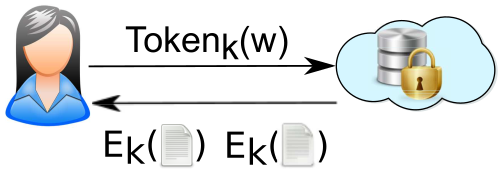
\includegraphics[width=0.4\linewidth]{images/encryption/token-based-search.png}
    \end{figure}
    \item \textbf{Crittografia omomorfica:} crittografia che supporta le operazioni direttamente sul cifrato
    \begin{figure}[ht]
        \centering
        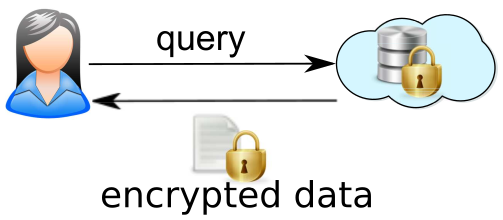
\includegraphics[width=0.4\linewidth]{images/encryption/homomorphic.png}
    \end{figure}
    \item \textbf{\textit{Encryption Schemas:}} ogni colonna può essere cifrata con un diverso schema crittografico 
    (\textit{random, add homomorphic, deterministic, order preserving, \dots})
    \begin{figure}[ht]
        \centering
        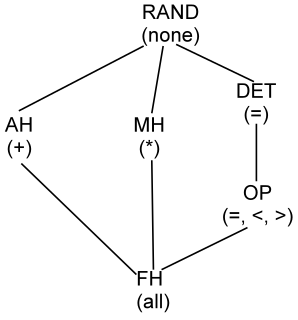
\includegraphics[width=0.3\linewidth]{images/encryption/schemas.png}
    \end{figure}
    \item \textbf{\textit{Onion Encryption:}} cifro i dati con diversi livelli \textit{a cipolla}, ognuno dei quali
    supporta l'esecuzione di una specifica \textit{query SQL}; l'idea è che \textit{scopro il dato solo quando mi serve}
    \begin{figure}[ht]
        \centering
        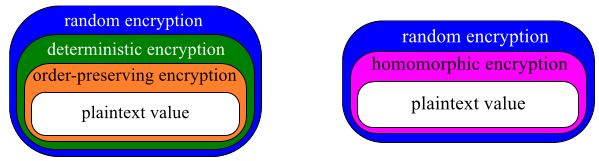
\includegraphics[width=0.8\linewidth]{images/encryption/onion.png}
    \end{figure}
    \item \textbf{Indicizzazione:} associo degli indici ai metadati
    \begin{figure}[ht]
        \centering
        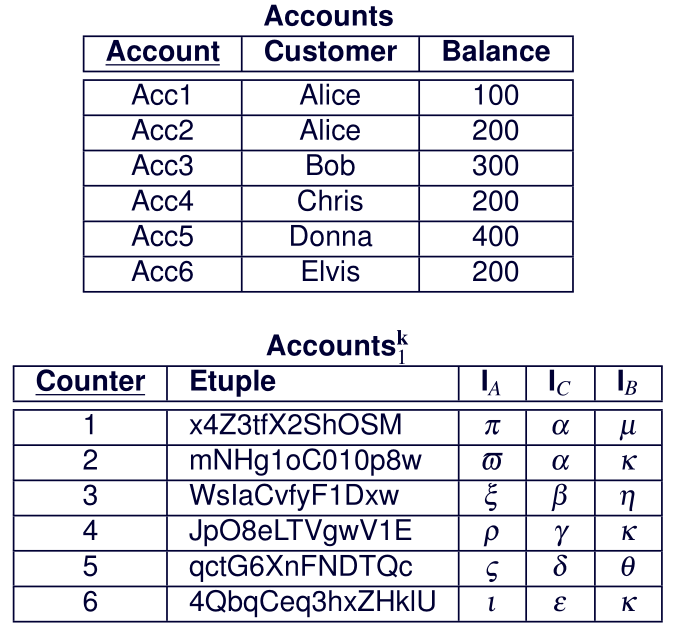
\includegraphics[width=0.6\linewidth]{images/encryption/indicizzazione.png}
    \end{figure}
    Nella seconda tabella: nella seconda colonna c'è la tupla criptata; nelle ultime tre ci sono gli attributi;
    si possono avere diversi tipi di indicizzazione:
    \begin{itemize}
        \item \textbf{\textit{Direct} $(1:1)$}
        
        \textcolor{darkgreen}{\textbf{+}} riesco a fare query precise
        
        \textcolor{red}{\textbf{-}} soggetto ad attacchi di frequenza
        \begin{figure}[ht]
            \centering
            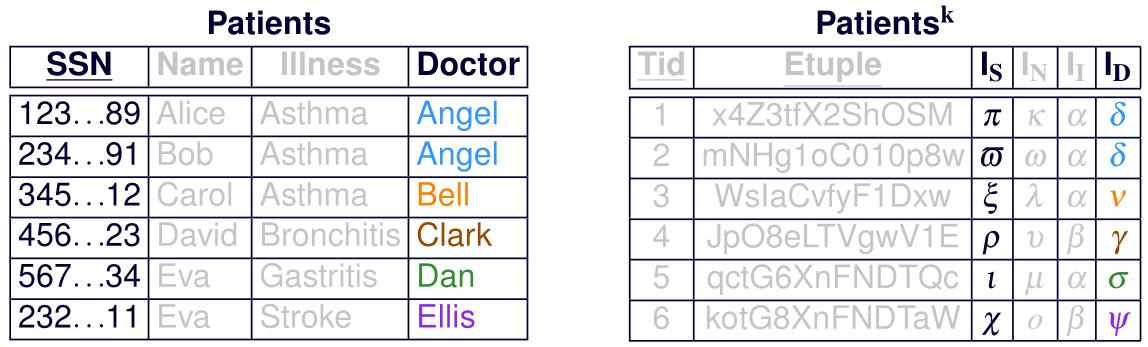
\includegraphics[width=0.85\linewidth]{images/encryption/index-direct.png}
        \end{figure}
        \item \textbf{\textit{Bucket} $(n:1) \rightarrow$} indicizzazione con collisione; ho diversi valori 
        che sono \textbf{mappati allo stesso indice}

        \textcolor{darkgreen}{\textbf{+}} non ho più attacchi di frequenze

        \textcolor{darkgreen}{\textbf{+}} supporta query di uguaglianza (\textit{se un valore è uguale ad un altro})
        
        \textcolor{red}{-} i risultati avranno delle tuple spurie

        \textcolor{red}{-} è ancora possibile fare qualche leakage
        \begin{figure}[ht]
            \centering
            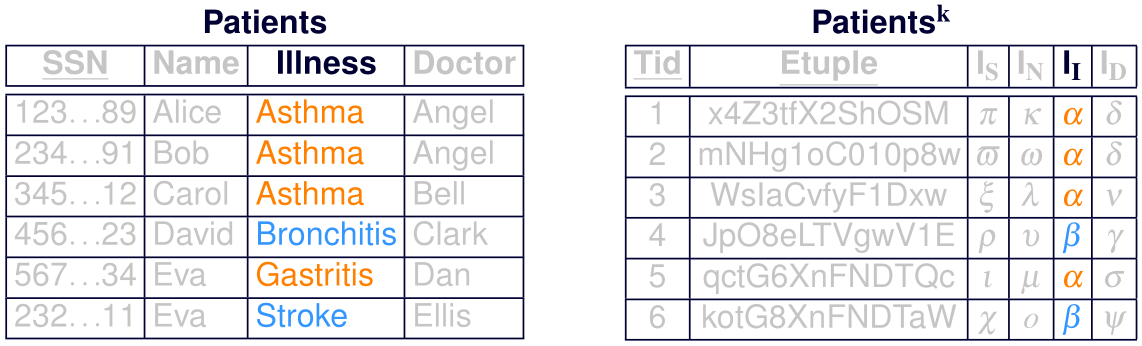
\includegraphics[width=0.85\linewidth]{images/encryption/bucket-index.png}
        \end{figure}
        \textit{In questo caso sono comunque esposto perché asma ha 3 occorrenze, dunque sarà per forza associata ad $\alpha$}

        \item \textbf{\textit{Flattened} $(1:n) \rightarrow$} ciascun indice deve avere lo stesso numero di occorrenze; significa che 
        i valori che hanno più occorrenze sono associati ad indici diversi

        \textcolor{darkgreen}{\textbf{+}} rimuovo la possibilità di fare attacchi di inferenze

        \textcolor{red}{\textbf{-}} sono esposto ad osservazioni dinamiche (magari certi dati sono sempre cercati assieme) 
        \begin{figure}[ht]
            \centering
            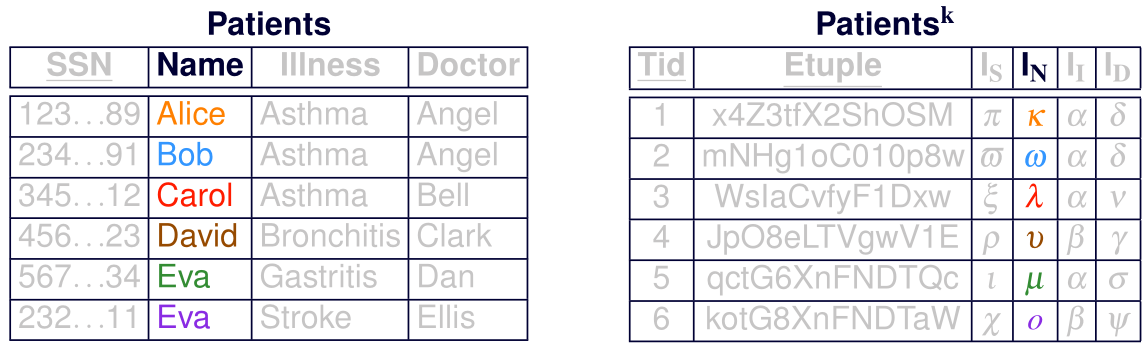
\includegraphics[width=0.85\linewidth]{images/encryption/flattened-index.png}
        \end{figure}

        \item \textbf{\textit{Partition-based:}}
        \begin{enumerate}
            \item si partiziona il dominio di un attributo
            \item a ciascuna partizione si assegna un'etichetta
            \item il valore in chiaro viene sostituito dall'etichetta
        \end{enumerate}

        \begin{figure}[ht]
            \centering
            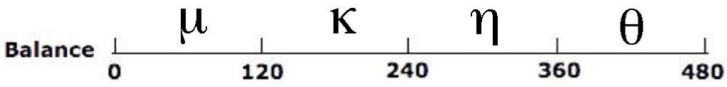
\includegraphics[width=0.6\linewidth]{images/encryption/partion-based-index.png}
        \end{figure}

        \noindent Supporta \textit{query} dove le condizioni sono espressioni booleane del tipo:

        - \textit{Attribute} \texttt{op} \textit{Value}

        - \textit{Attribute} \texttt{op} \textit{Attribute}

        dove \texttt{op}$=\{ =, <, >, \leq, \geq \}$

        \begin{figure}[ht]
            \centering
            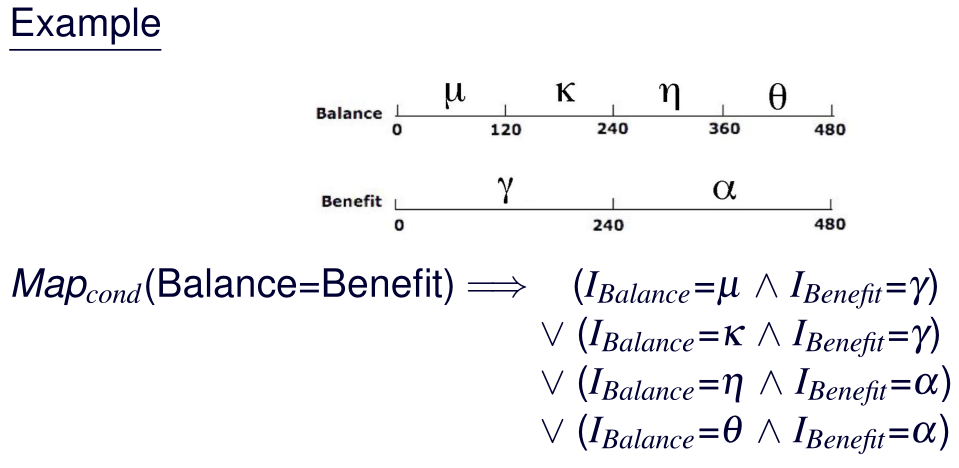
\includegraphics[width=0.6\linewidth]{images/encryption/partition-based-ex.png}
        \end{figure}

        \noindent \textbf{Esecuzione delle query:}

        \noindent Ogni query $Q$ sul DB in chiaro viene tradotta in:
        \begin{enumerate}
            \item una query $Q_s$ da eseguire sul server $\rightarrow$ query sull'indice per ottenere le tuple criptate
            \item una query $Q_c$ da eseguire sul client $\rightarrow$ decriptare il risultato della query precedente e filtrare le tuple spurie
        \end{enumerate}

        La traduzione dovrebbe essere fatta in modo tale che il server sia responsabile 
        della maggior parte del lavoro.

        \begin{figure}[ht]
            \centering
            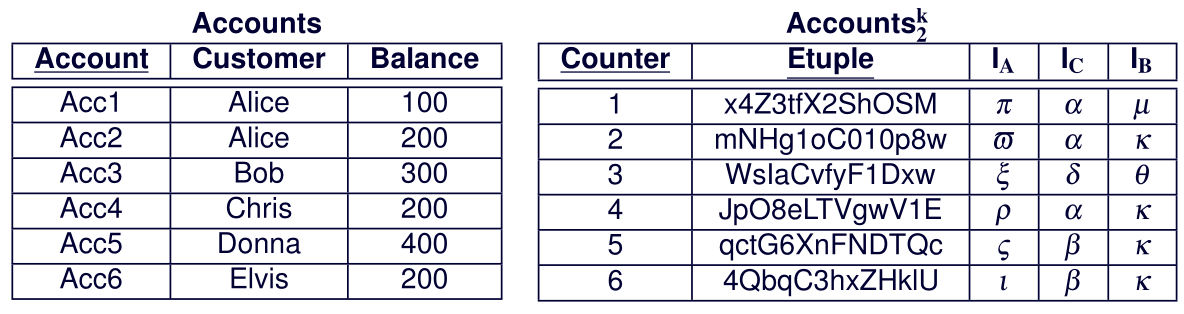
\includegraphics[width=0.8\linewidth]{images/encryption/query-ex-1.png}
        \end{figure}
        \begin{figure}[ht]
            \centering
            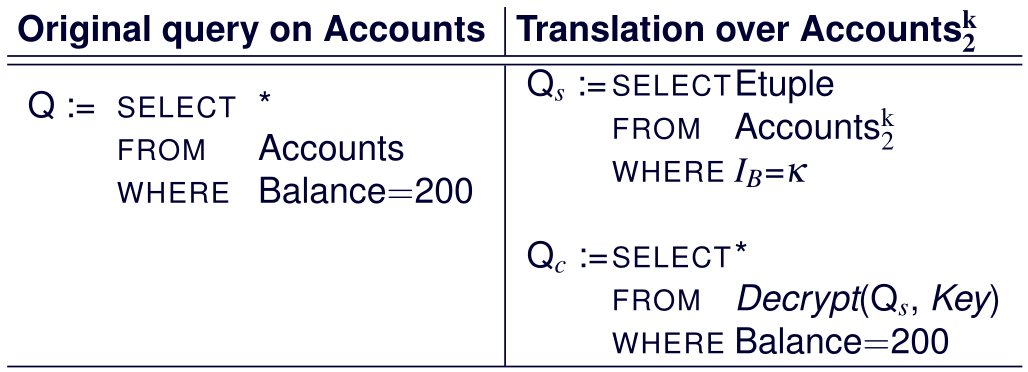
\includegraphics[width=0.8\linewidth]{images/encryption/query-ex-2.png}
        \end{figure}

        \newpage
        \item \textbf{\textit{Hash-based:}} basate sul concetto di \textit{one-way hash function}; ogni
        attributo viene mappato ad un indice utilizzando una funzione di hash sicura.

        \noindent Dat una funzione $h$ e il dominio degli attributi $D_i$, diciamo che $h$ è \textbf{sicura} se:
        \begin{enumerate}
            \item $\forall x, y \in D_i \implies h(x) = h(y)$ (\textbf{determinismo}) 
            \item dati due valori $x, y \in D_i$ tali che $ x \neq y$, potremmo avere che $h(x)=h(y)$ (\textbf{collisione}, per proteggermi da attacchi di frequenza)
            \item la distanza dei valori in chiaro deve essere \textbf{indipendente} dalla distanza dei valori di hash (\textit{strong mixing})
        \end{enumerate}

        \noindent Questo metodo supporta \textit{query} dove le condizioni sono espressioni booleane del tipo:
        \begin{itemize}
            \item $ Attribute = Value$
            \item $Attribute_1 = Attribute_2$, se sono indicizzati con la stessa funzione di hash
        \end{itemize}
        
        \noindent La traduzione funziona come nel metodo \textit{partion-based}; non 
        sono supportate \textit{query di range}. 
    \end{itemize}
\end{itemize}

\subsubsection{Interval-based queries}
\begin{itemize}
    \item Le tecniche di indicizzazione che preservano l'ordine supportano 
    query di range, ma sono esposte ad inferenza
    \item Le tecniche di incizzazione che \textit{non} preservano l'ordine non sono esposte 
    ad inferenza, ma non supportano query di range
\end{itemize}

$\rightarrow$ viene calcolato un $B_+ -tree$ dal client, ed ogni nodo viene criptato come un tutt'uno; successivamente 
per rispondere alle query l'albero viene visitato (in ambiente trusted).

\newpage
\section{\textit{Searchable Encryption}}
\subsection{\textit{Order preserving encryption}}
\begin{itemize}
    \item \textbf{\textit{Order Preserving Encryption Schema (OPES):}} prende in input una distribuzione target 
    di valori per gli indici ed applica una trasformazione che preserva l'ordine e rispecchia 
    la distribuzione di input.

    \textcolor{darkgreen}{\textbf{+}} la comparazione può essere fatta direttamente sui dati criptati 

    \textcolor{darkgreen}{\textbf{+}} le query non producono tuple spurie 

    \textcolor{red}{\textbf{-}} vulnerabile ad attacchi di inferenza

    \item \textbf{\textit{Order Preserving Encryption with Splitting and Scaling (OPESS):}}
    
    Questo schema crea degli indici in modo tale che la loro distribuzione delle frequenze sia piatta.
\end{itemize}

\subsection{\textit{Fully homomorphic encryption}}

\begin{itemize}
    \item Permette una performante computazione specifica sui dati criptati 
    \item Decriptando il risultato, si ottiene lo stesso risultato delle stesse operazioni sui dati in chiaro
\end{itemize}

\newpage
\section{Esposizione all'inferenza}

Ci sono due requisiti conflittuali quando si parla di 
\textit{indicizzare} dati:
\begin{itemize}
    \item gli indici dovrebbero fornire una \textbf{esecuzione delle query efficiente}
    \item gli indici non dovrebbero aprire porte ad attacchi di \textbf{inferenza} e \textit{linking}
\end{itemize}

$\rightarrow$ diventa importante misurare quantitativamente il livello di esposizione dovuto 
alla pubblicazione degli indici:

\centering $\epsilon =  $ \textit{Coefficiente di Esposizione}

\noindent La computazione del \textit{Coefficiente di Esposizione} dipende da diversi fattori:
\begin{itemize}
    \item \textbf{Metodo di incizzazione utilizzato}
    \begin{itemize}
        \item \textit{direct encryption}
        \item \textit{hashing}
    \end{itemize}
    \item \textbf{Conoscenza pregressa dell'attaccante}
    \begin{itemize}
        \item $Freq + DB^k$
        \item $DB + DB^k$
    \end{itemize}

    \noindent In entrambi i casi l'attaccante può risalire alla funzione di incizzazione.
\end{itemize}

\raggedright

\subsection{Direct Encryption}
\subsubsection{\textbf{Freq + $DB^k$}}

\begin{itemize}
    \item La corrispondenza tra indice e valore in chiaro può essere determinata sulla base 
    del numero di occorenze di indice/valore

    $\rightarrow$ \textbf{Protezione base:} i valori con lo stesso numero di occorenze sono indistinguibili per l'attaccante
    \item Valutazione dell'esposizione dell'indice basata sulla relazione di equivalenza
    in cui i valori di indice/valore con lo stesso numero di occorrenze
    appartengono alla stessa classe

    $\rightarrow$ L'esposizione di un indice nella classe di equivalenza $C$ è $1 / |C|$ 
\end{itemize}

\begin{figure}[ht]
    \centering
    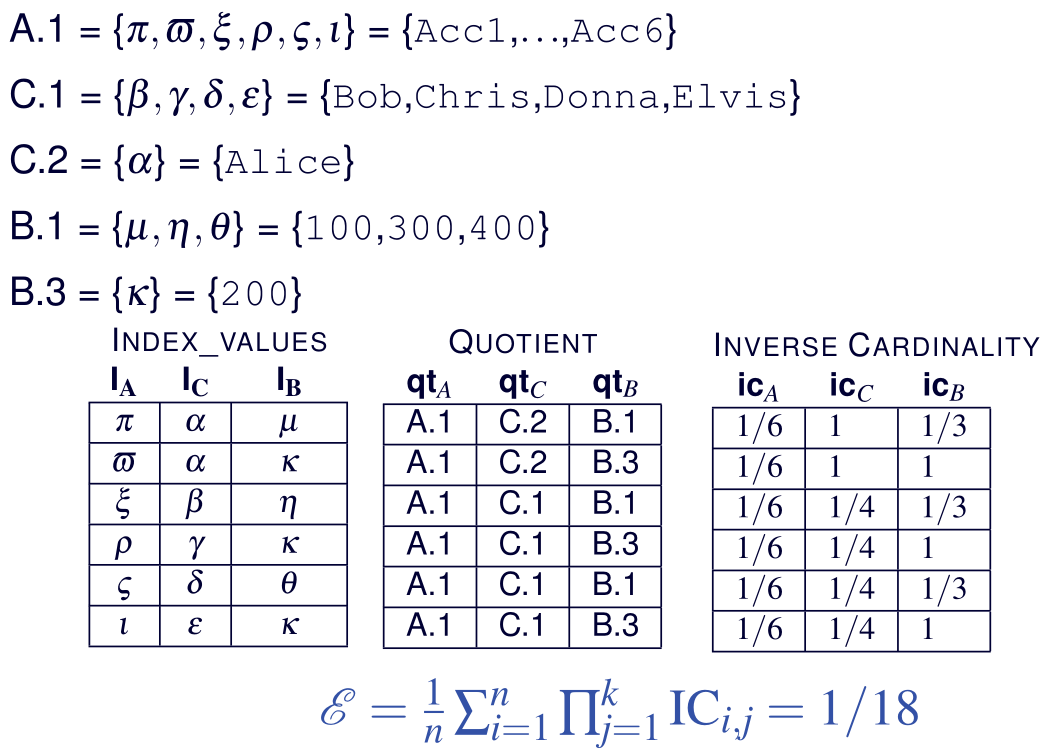
\includegraphics[width=0.9\linewidth]{images/encryption/direct-freq-db.png}
\end{figure}

\newpage
\begin{itemize}
    \item nella tabella \textit{Quotient} ci sono le classi di equivalenza a cui appartengono gli indici
    \item nella tabella \textit{Inverse Cardinality} c'è $1/|C|$ , si interpreta come:
    \begin{itemize}
        \item \textit{c'è 1 di 6 valori che non so distinguere}
        \item \textit{c'è 1 di 4 valori che non so distinguere}
        \item Sta esprimendo l'incertezza; più sarà grande $|C|$, più avrò incertezza 
        
        $\rightarrow$ quelli con $1/1$ rappresentano un problema dato che non c'è incertezza
    \end{itemize}
    \item A \textbf{livello di tupla} l'incertezza è il \textbf{prodotto} delle incertezze
    \item A \textbf{livello di tabella} faccio la \textbf{media} dell'esposizione delle tuple ($\epsilon$)
\end{itemize}

\subsubsection{DB + $DB^k$}
\begin{itemize}
    \item Grafo \textbf{\textit{Row-Column-Value}} non-direzionato a 3 colori
    \begin{itemize}
        \item un vertice di colore \textit{column} per ogni attributo 
        \item un vertice di colore \textit{row} per ogni tupla 
        \item un vertice di colore \textit{value} per ogni valore distinto in una colonna
        \item un arco connette ogni valore alla riga e colonna in cui compare
    \end{itemize}
    \item RCV sui valori in chiaro è uguale a quello sugli indici
    \item posso avere una misura del grado di esposizione guardando quanto \textit{un nodo si confonde} (automorfismo)
\end{itemize}

\begin{figure}[ht]
    \centering
    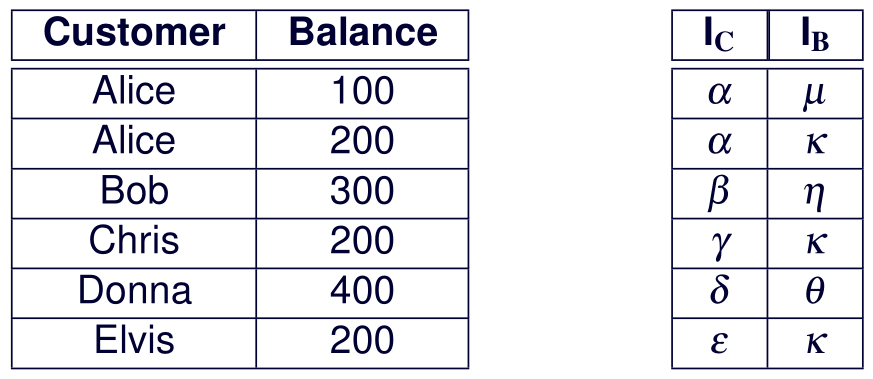
\includegraphics[width=0.7\linewidth]{images/encryption/direct-db-dbk1.png}
\end{figure}
\begin{figure}[ht]
    \centering
    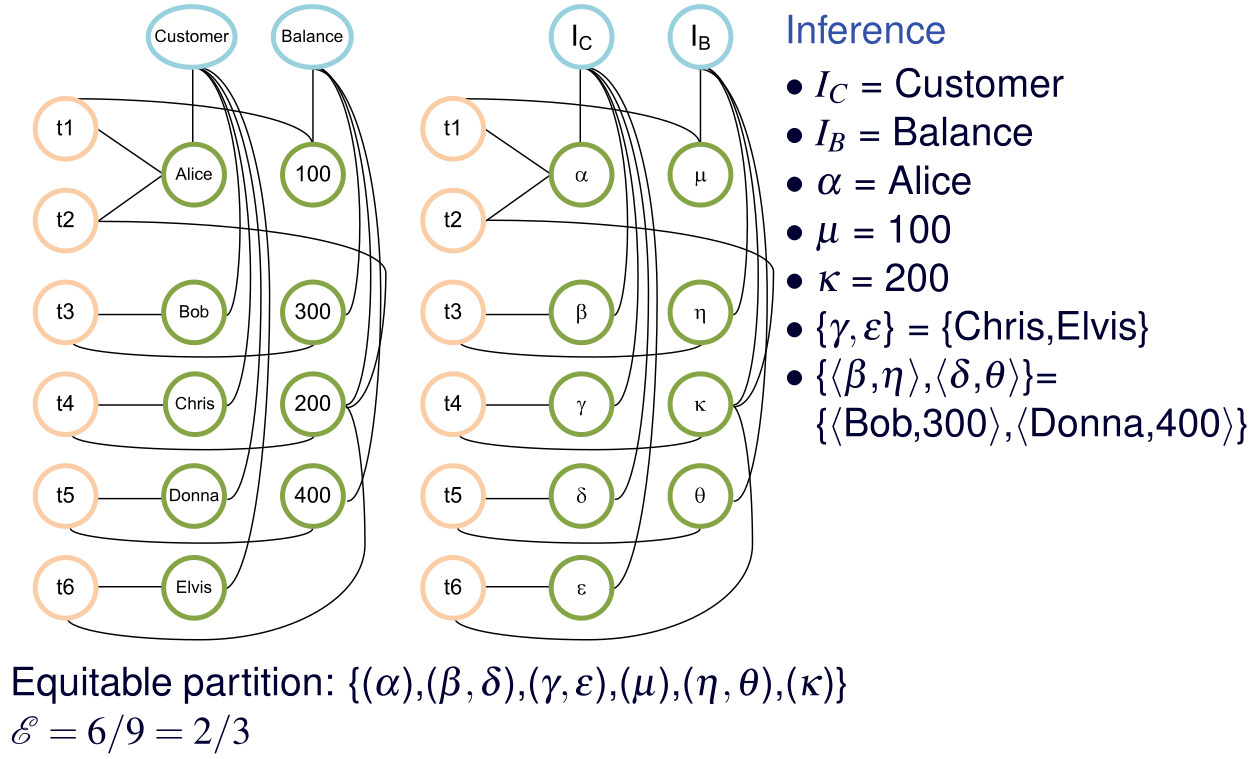
\includegraphics[width=1\linewidth]{images/encryption/direct-db-dbk2.png}
\end{figure}

\newpage
Per \textit{Equitable Partion} si intende un insieme di vertici che costituiscono un automorfismo.

\noindent L'esposizione si calcola come il rapporto tra il numero di \textit{equitable partition} e il numero totale degli elementi.

\newpage
\subsection{Hashing}
\subsubsection{Freq + $DB^k$}
\begin{itemize}
    \item La funzione di hash è caratterizzata da un \textit{fattore di collisione}, ovvero il numero 
    di valori che in media collidono sullo stesso indice 
    \item Sono possibili diversi mapping dei valori negli indici, in relazione ai vincoli imposti dalle frequenze 
    \item Per ogni mapping si calcola il coefficiente di esposizione
\end{itemize}

\subsubsection{DB + $DB^k$}
\begin{itemize}
    \item i grafi RCV tra dati in chiaro e criptati non sono uguali, dato che \textit{vertici diversi} nel grafo in chiaro 
    potrebbro collassare nello \textit{stesso vertice} nel grafo criptato
    \item il numero di archi che collega i vertici \textit{row} ai vertici \textit{value} è lo stesso
    \item il problema diventa trovare un \textit{matching corretto} tra gli archi del grafo in chiaro e quello criptato
\end{itemize}

\newpage
\section{Bloom Filter}
Il \textit{Bloom Filter} sta alla base della costruzione di alcune tecniche 
di indicizzazione; è un metodo efficiente per codificare l'appartenenza a un insieme.

\begin{itemize}
    \item set di $n$ elementi ($n$ è grande)
    \item vettore di $l$ bit ($l$ è piccolo)
    \item $h$ funzioni di hash indipendenti $H_i : \{0,1\}^* \rightarrow [1,l]$
    \item \textbf{Insert x:} set a 1 i bit corrispondenti a $H_1(x), H_2(x), \dots, H_h(x)$
    \item \textbf{Search x:} Computare $H_1(x), H_2(x), \dots, H_h(x)$ e verificare se quei valori sono settati a 1 nel vettore
\end{itemize}

\begin{figure}[ht]
    \centering
    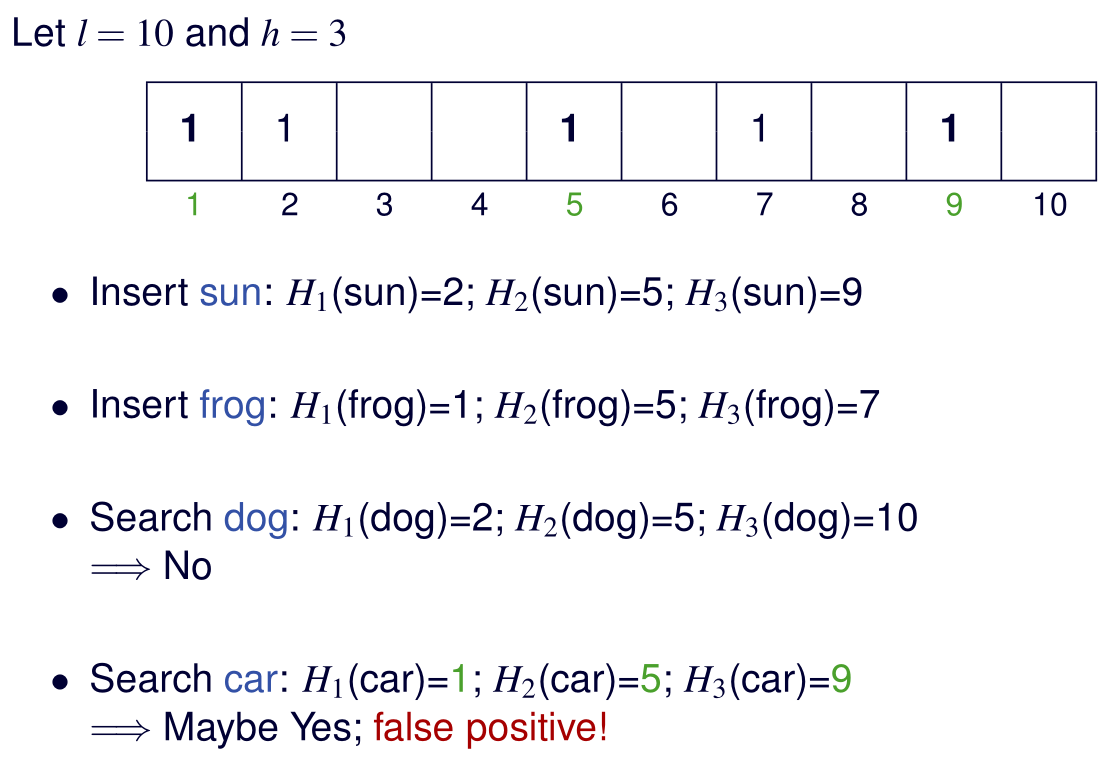
\includegraphics[width=0.8\linewidth]{images/encryption/bloom-filter.png}
\end{figure}

\begin{itemize}
    \item è una generalizzazione dell'hashing (\textit{bloom filter} con 1 funzione di hash equivale all'hash ordinario)
    
    \textcolor{darkgreen}{\textbf{+}} efficiente nello spazio
    
    \textcolor{red}{\textbf{-}} gli elementi non possono essere rimossi

    \item ha una costante di probabilità di ottenere un falso positivo

    \textcolor{red}{\textbf{-}} teoricamente non accettabile 

    \textcolor{darkgreen}{\textbf{+}} nella pratica è accettabile perché il costo viene messo in relazione ai guadagni in termini di spazio
\end{itemize}

\newpage
\section{Integrità dei Dati}
Due aspetti:
\begin{itemize}
    \item \textbf{Integrità in Storage:} i dati devono essere protetti da modifiche non autorizzate
    
    $\rightarrow$ update non autorizzate devono essere rilevati
    \begin{itemize}
        \item si ottiene utilizzando la \textbf{firma digitale} a livello di tupla (a livello di cella sarebbe troppo costoso)
    \end{itemize}

    \item \textbf{Integrità nelle query:} i risultati delle query devono essere corretti e completi
    
    $\rightarrow$ un comportamento non corretto del server deve essere rilevato
\end{itemize}

\section{\textit{Selective-Encryption} e \textit{Over-Encryption}}
Utenti diversi potrebbero necessitare di viste diverse dei dati nel cloud

$\rightarrow$ \textbf{Selective Encryption:} la politica di autorizzazione definita dal proprietario dei dati 
viene tradotta in una politica di encryption equivalente

\begin{figure}[ht]
    \centering
    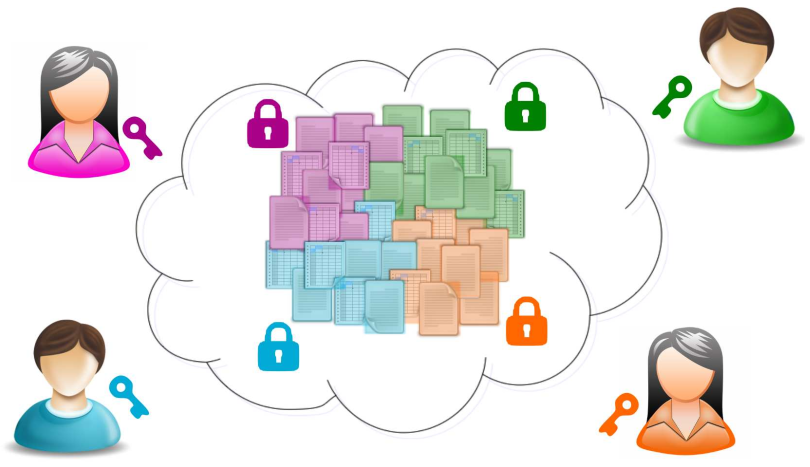
\includegraphics[width=0.7\linewidth]{images/encryption/selective.png}
\end{figure}

\textit{Desiderata:}
\begin{itemize}
    \item i dati stessi dovrebbero regolare i controlli di accesso 
    \item dovrebbero essere usate chiavi differenti per criptare i dati 
    \item l'autorizzazione di accesso a una risorsa viene tradotta nella \textbf{conoscenza della chiave} con cui la risorsa è criptata 
    \item ad ogni utente vengono comunicate le chiavi per decriptare i dati a cui ha diritto di accesso
\end{itemize}

\subsubsection{Politiche di Autorizzazione}
Il \textit{data owner} definisce delle politiche di autorizzazione per regolare l'accesso ai dati.

\begin{itemize}
    \item Una politica di autorizzazione $\mathcal{A}$ è un set di permessi della forma $\left\langle user, resource \right\rangle$
    
    \noindent Può essere rappresentata sotto forma di:
    \begin{itemize}
        \item matrice 
        \item grafo diretto bipartito
    \end{itemize}
    \item L'idea è che diverse autorizzazioni di accesso ai dati implicano diverse chiave per criptare 
\end{itemize}

\begin{figure}[ht]
    \centering
    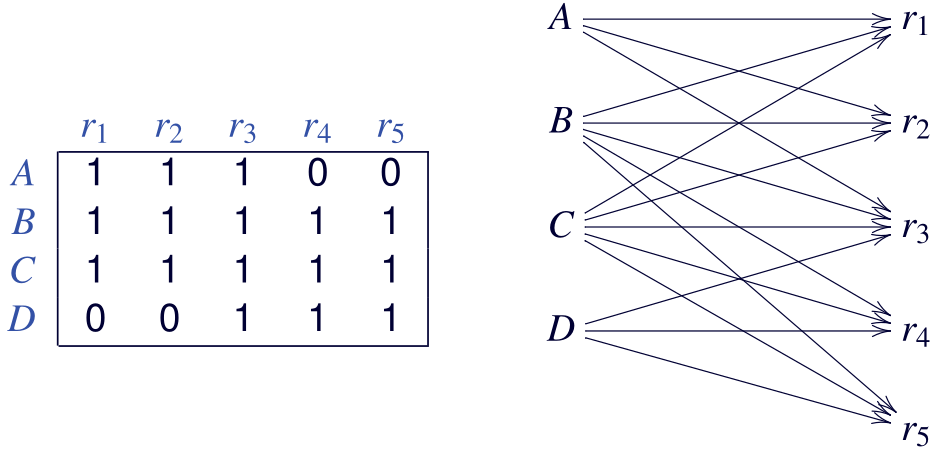
\includegraphics[width=0.7\linewidth]{images/encryption/auth-policy.png}
\end{figure}

\subsubsection{Politica di Encryption}
La \textit{politica di autorizzazione} definita dal data owner viene tradotta
in una \textit{politica di encyption} equivalente.

\noindent Due possibili soluzioni:
\begin{itemize}
    \item criptare ogni risorsa con una chiave diversa e dare all'utente le chiavi 
    che decriptano le risorse a cui ha accesso 

    \textcolor{red}{\textbf{-}} l'utente deve gestire tante chiavi quante sono le risorse a cui ha accesso
    \item usare un \textbf{metodo di derivazione delle chiavi} per permettere di derivare dalla propria chiave utente 
    tutte le chiavi a cui hanno accesso 

    \textcolor{darkgreen}{+} ad ogni utente viene rilasciata una sola chiave
\end{itemize}

\subsubsection{Metodi di Derivazione delle Chiavi}
\begin{itemize}
    \item Basata sulla definizione di una \textbf{gerarchia di derivazione delle chiavi} $(\mathcal{K}, \leq)$
    \begin{itemize}
        \item $\mathcal{K}$ è il set di chiavi 
        \item $\leq$ è la relazione d'ordine parziale definita su $\mathcal{K}$
    \end{itemize}
    \item $(\mathcal{K}, \leq)$ può essere rappresentata come un grafo con un vertice per ogni $x \in \mathcal{K}$ e un percorso da $x$ a $y$ sse $y \leq x$
\end{itemize}

\subsubsection{Metodi di Derivazione delle Chiavi basati su Token}
\begin{itemize}
    \item Le chiavi sono assegnate arbitrariamente ai vertici 
    \item Una label $l_i$ (pubblica) viene assegnata a ciascuna chiave $k_i$
    \item Un token $t_{i,j}$ (pubblico) viene associato ad ogni arco nella gerarchia
    \item Dato un arco $(k_i, k_j)$, il token $t_{i,j}$ viene calcolato come $k_j \oplus h(k_i, l_j)$, dove:
    \begin{itemize}
        \item $\oplus$ è l'operatore \texttt{xor}
        \item $h$ è una funzione di hash sicura
    \end{itemize}
    \item \textcolor{darkgreen}{\textbf{+}} i token sono pubblici e permettono agli utenti di derivare più chiavi, ma dovendosi preoccupare solo di una 
    \item \textcolor{darkgreen}{\textbf{+}} possono essere storati su un server così che ogni utente vi può accedere
\end{itemize}

\noindent Le relazioni delle chiavi tramite token possono essere rappresentate con un grafo:
\begin{itemize}
    \item un vertice per ogni coppia $\left\langle k, l \right\rangle$, dove $k \in \mathcal{K}$ è una chiave e $l \in \mathcal{L}$ è l'etichetta associata 
    \item un arco dal vertice $\left\langle k_i, l_i \right\rangle$ a $\left\langle k_j, l_j \right\rangle$ se esiste un token $t_{i,j} \in \mathcal{T}$ che permette la derivazione di $k_j$ a partire da $k_i$
\end{itemize}

\begin{figure}[ht]
    \centering
    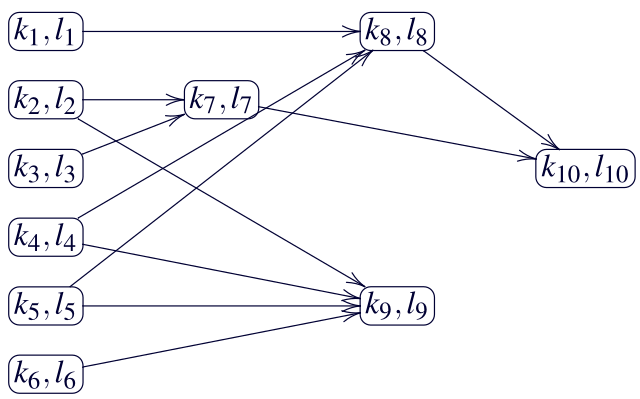
\includegraphics[width=0.6\linewidth]{images/encryption/token-based-ex.png}
\end{figure}


\noindent Traduzione della politica di autorizzazione in una di encryption:
\begin{itemize}
    \item \textit{Desiderata:}
    \begin{itemize}
        \item ad ogni utente viene rilasciata una sola chiave 
        \item le risorse vengono criptate una sola volta con una sola chiave 
    \end{itemize}
    \item Una funzione $\phi : \mathcal{U} \cup \mathcal{R} \rightarrow \mathcal{L}$ che descrive:
    \begin{itemize}
        \item l'associazione tra un utente la (etichetta della) sua chiave
        \item l'associazione tra una risorsa e la (etichetta della) chiave usata per criptarla
    \end{itemize}
\end{itemize}

\subsubsection{Definzione Formale della Politica Crittografica}
Una \textbf{politica di encryption} su utenti $\mathcal{U}$ e risorse $\mathcal{R}$, denotata come $\mathcal{E}$,
è una 6-tupla $\left\langle \mathcal{U, R, K, L, \phi, T} \right\rangle$, dove:
\begin{itemize}
    \item $\mathcal{K}$ è il set di chiavi del sistema e $\mathcal{L}$ l'insieme delle chiavi corrispondenti
    \item $\phi$ è la funzione di assegnamento delle chiavi e schema crittografico 
    \item $\mathcal{T}$ è il set di token definiti su $\mathcal{K}$ e $\mathcal{L}$
\end{itemize}

\noindent La politica di encryption può essere rappresentata come un grafo estendo quello di chiavi 
e token per includere:
\begin{itemize}
    \item un vertice per ogni utente e ogni risorsa 
    \item un arco da ogni vertice utente $u$ a $\left\langle k, l \right\rangle$ tale che $\phi(u)=l$
    \item un arco da ogni vertice $\left\langle k, l \right\rangle$ a ogni vertice risorsa $r$ tale che $\phi(r)=l$
\end{itemize}

\begin{figure}[ht]
    \centering
    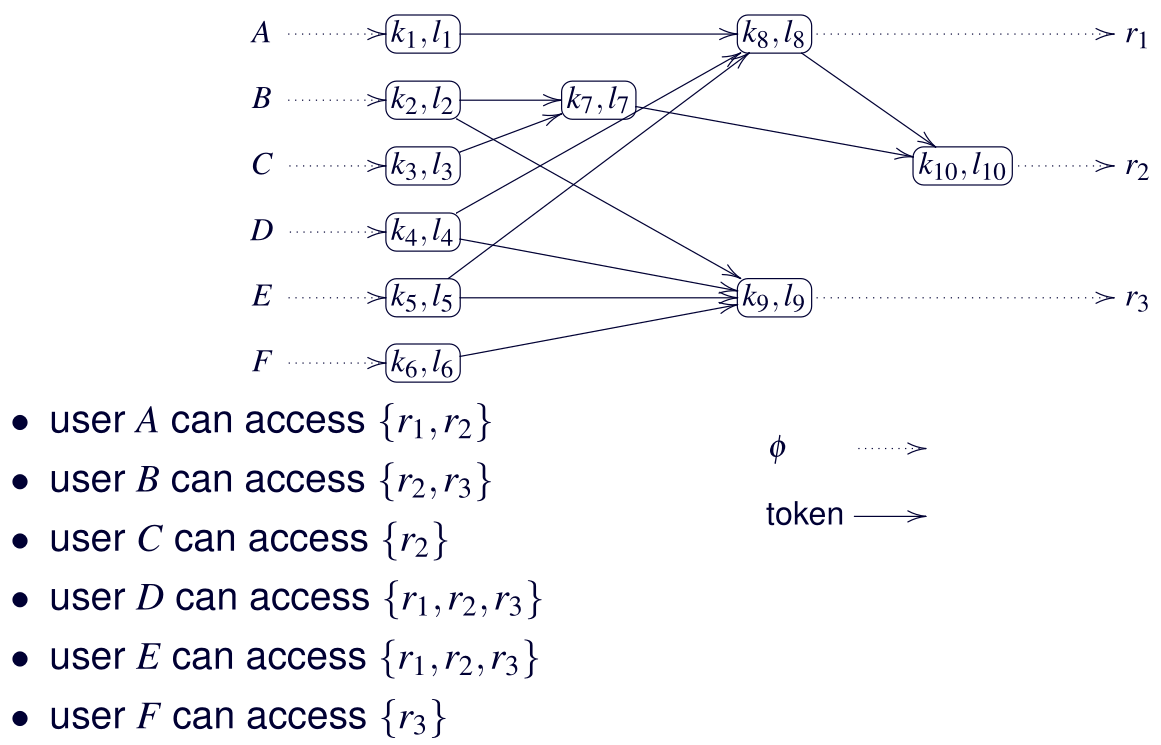
\includegraphics[width=1\linewidth]{images/encryption/encryption-policy-graph.png}
\end{figure}














\end{document}